%! Author = Saeid Yazdani
%! Date = 1/6/2024


\section{Design for Manufacturability}
\label{sec:dfm}

One of the essential aspects of \ac{DfX} is \ac{DfM},
which constitutes the basis for high \emph{Functional Yield},
and \emph{Parametric Yield} that
specifies an acceptable band in which the product should be in terms of
performance \autocite{4145590}.
\ac{DfM} summarizes concepts that guarantee low-stress manufacturing in
order to keep yield high and fabrication pre-damage low.

There is a tight coupling between \ac{DfM} and \ac{DfR}:
Even if the design rule specified dimensions
turn out to be functional during production and assembly, the headroom for
surviving stress during lifetime will most likely be significantly less.

\begin{figure}[h]
    \centering
    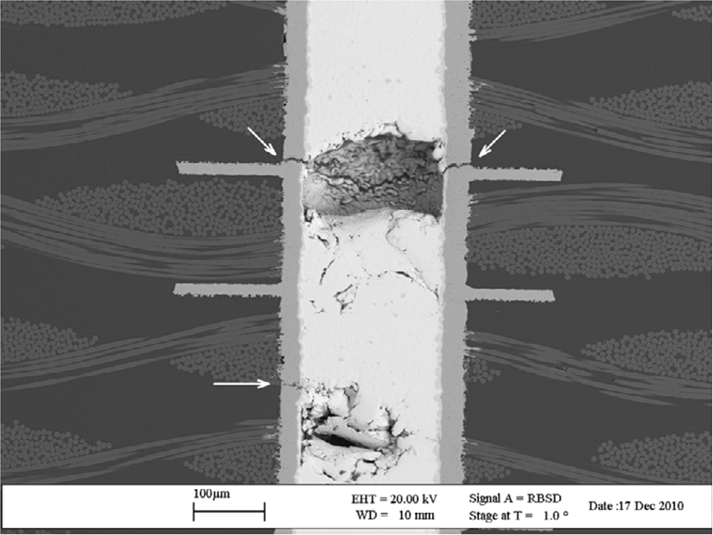
\includegraphics[scale=0.28]
    {figures/via-barrel-crack}
    \caption[Plated-Through Via crack]
    {Cross-section of a \ac{PTH} via that has developed micro-cracks due to
    thermal stress \autocite{5898628}.}
    \label{fig:example-pth-via-crack}
\end{figure}


On the other hand, the value obtained from \ac{DfM} is a tested and
measured number and will result in a better yield.

There are two major categories of \ac{DfM} in electronic industry
with similar concepts but different execution:
\emph{\ac{DfM} for \acp{IC}} and \emph{\ac{DfM} for board-level and
system-level}.

\ac{DfM} is evolving continuously due to advancements in
process techniques and capabilities of the manufacturing industry,
as many of the production problems have been solved over time.

\subsection{\ac{DfM} at Silicon-Level}
\label{subsec:dfm-ic}

\ac{DfM} guidelines for \ac{IC} fabrication are aimed at increasing yield and
achieving desired performance levels (parametric yield).
As stated before, the guidelines are just an addition to industry standard
design rules and manufacturer specifications to produce a better result at the
fab production line.

A few examples of \ac{DfM} guidelines in the context of silicon production
are given below:

\begin{itemize}[topsep=8pt,itemsep=4pt,partopsep=4pt, parsep=4pt]

    \item Respecting manufacturing tolerances of equipment is vital in
    production line throughput

    \item Keeping \acp{CD} unchanged over the whole wafer area will help
    to achieve uniform parametric yield.
    \ac{OPC} can offer pattern printability and
    quality \autocite{5755022}.

    \item Sticking to basic shapes will result in higher yields when
    compared to complex, hard-to-print shapes.

    \item Knowing exposure times will help to avoid distortions due to
    over-extended exposure times.

\end{itemize}

\subsection{\ac{DfM} at Board-Level}
\label{subsec:dfm-pcb}

At the board level, \ac{DfM} guidelines are mainly focused on generating optimal
yield in the assembly line and achieving maximum functional performance for the
product.
This includes provisioning for mechanical stress during production (solder
stress, shear or cutting stress, mechanical assembly stress) and signal
integrity during application.

A few examples of \ac{DfM} guidelines in the context of electronic systems are
given below:

\begin{itemize}[topsep=4pt,itemsep=2pt,partopsep=2pt, parsep=2pt]

    \item \textbf{\emph{\ac{PCB} Layout}:}
    \begin{itemize}[topsep=4pt,itemsep=2pt,partopsep=2pt, parsep=2pt]

        \item Respecting manufacturing tolerances such as drill
        hole size and minimum distances between elements (via to via, trace to
        via, etc., for safe insulation and no arcing).

        \item  Respecting manufacturing limitations of via holes – especially
        in the case of multi-layer boards with risky sidewall plating of via
        connections and risky soldering because of the Z swelling in multi-layer
        boards.

        \item Check for the maximum current density in wires and via holes, even
        in the case of emergency operation (shorts in power supplies: the wire
        should survive the time to fusing).

        \item To ensure signal integrity, attention should be given to the
        vicinity of high power, high frequency, and other \ac{RF} traces and
        components.

    \end{itemize}

    \item \textbf{\emph{Component Placement}:}
    \begin{itemize}[topsep=4pt,itemsep=2pt,partopsep=2pt, parsep=2pt]

        \item Component placement is crucial to reliability and lifetime.
        The placement must guarantee low mechanical stress during shock events
        or vibration, and we must add just enough supporting posts to keep
        component movement at a minimum.

        \item Clearance from edges is vital for manufacturing and
        handling during assembly.

        \item Weight distribution is an essential factor for assembly. The best
        case is that the weight is evenly distributed across a board.

        \item Adequate spacing between components should be respected and
        ideally components with high heat and \ac{RF} radiation should be away
        as far as possible to components which are susceptible to heat and
        \ac{RF} radiation to reduce risks of lifetime reduction or performance
        degradation.

        \item Placement of large and small components in tight vicinities
        makes assembly and future repairs and reworks difficult.

    \end{itemize}

    \item \textbf{\emph{Component Soldering}:}
    \begin{itemize}[topsep=4pt,itemsep=2pt,partopsep=2pt, parsep=2pt]

        \item Footprint in the layout must correspond to the type of soldering
        (\emph{reflow} or \emph{wave} soldering). In addition, for smaller
        \ac{SMD} components,
        design of thermal relief and vicinity from power planes can prevent
        common problems such as cold solder joints and tombstoning
        (\autoref{fig:example-tombstone}) of \ac{SMD} components.

        \begin{figure}[h]
            \centering
            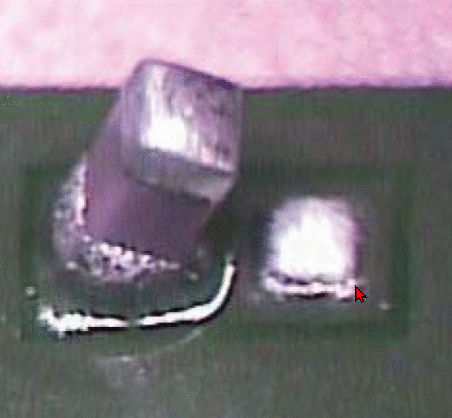
\includegraphics[scale=0.35]
            {figures/tombstoned-cap}
            \caption[Example of Tombstone in \acs{SMD} Components]
            {Optical image of a \emph{0201} sized capacitor suffering from
            tombstone after solder reflow \autocite{6243196}.}
            \label{fig:example-tombstone}
        \end{figure}

        \item If large and small components are placed very close to each other,
        the larger components and their footprint can absorb most of the
        soldering heat, thereby leaving less chance for smaller components in
        their vicinity to be soldered correctly.
        This should be addressed at the placement time.

        \item Placement of large and small components in tight vicinities
        makes assembly and future repairs and reworks difficult.

        \item  In the case of a two-sided assembly, the first and
        second runs of the solder process are defined in a way that
        small components are placed on the side that is
        supposed to be the \emph{first} solder run, as
        only lightweight components can be held securely in place when hanging
        top-down underneath the board during the second soldering run.
        \paragraph{}{ On the other hand, it should be noted that
        there is a risk of solder rejection
        coming from the heat resistant glue that keeps SMT devices in
        place in a solder bath in the case of wave soldering.}

    \end{itemize}

\end{itemize}
